
\section{Verificación}

En este primer apartado se verifica la solución obtenida con el DVM. Se ha escogido el perfil NACA 2408 sin deflexión de flap de borde de salida y con un ángulo de ataque $\alpha = 4  \degrees$. Para ello se analiza la convergencia del coeficiente de sustentación $\left( C_{l} \right)$ y el coeficiente de momento respecto del borde de ataque $\left( C_{m,\text{LE}} \right)$. Posteriormente se comparan los resultados obtenidos del DVM con los calculados de la TAT.

\begin{figure}[h]
    \centering
    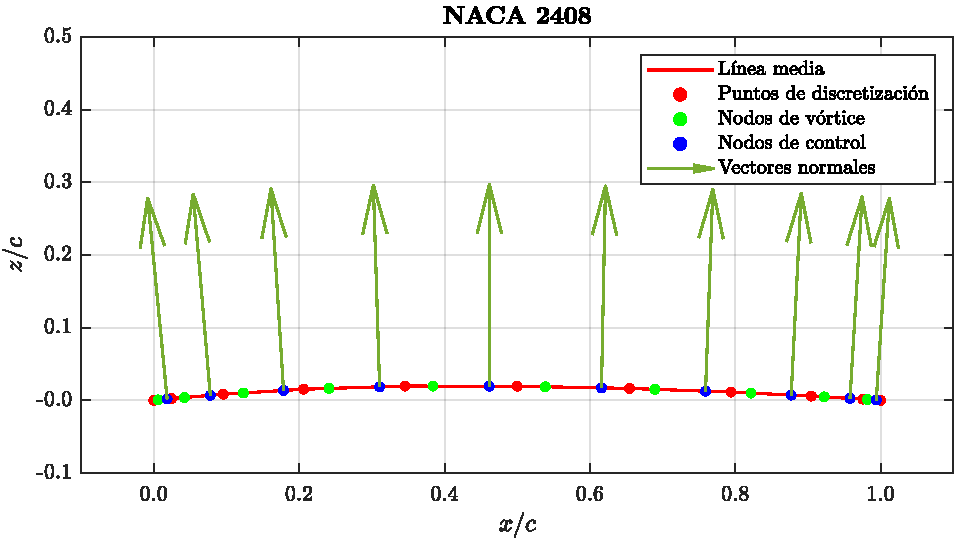
\includegraphics[width=\linewidth]{imagenes/verificacion/verificacion_perfil.pdf}
    \caption{Línea media, puntos de discretización, nodos de vórtice, nodos de control y vectores normales para el perfil NACA 2408 sin flap de borde de salida, con distribución \emph{full cosine} y $N = 10$ paneles.}
    \label{fig:verificacion_perfil}
\end{figure}

El coeficiente de sustentación se calcula para distintos números de paneles $\left( 0 - 200 \right)$. En la figura \ref{fig:verificacion_perfil} se representa la línea media del perfil NACA 2408, la separación entre paneles, las posiciones de los vórtices, los puntos de control y los vectores normales.

\begin{figure}[ht] 
    \centering
    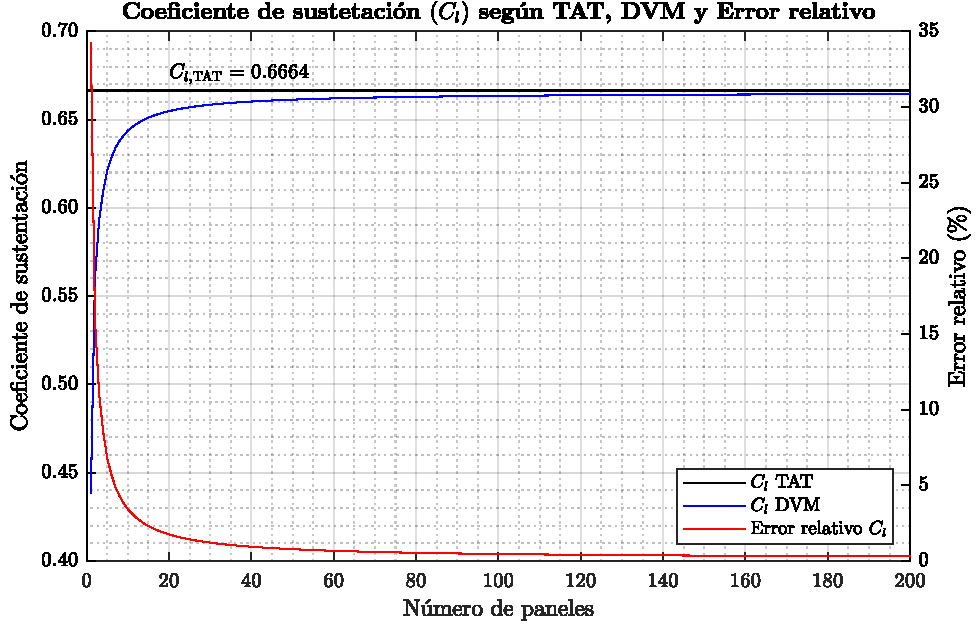
\includegraphics[width=\linewidth]{imagenes/verificacion2/verificacion_cl.pdf}
    \caption{Coeficiente de sustentación $\left( C_l \right)$ según TAT, DVM y error relativo en función del número de paneles $\left( N \right)$.}
    \label{fig:verificacion_cl}
\end{figure}

\begin{figure}[ht]
    \centering
    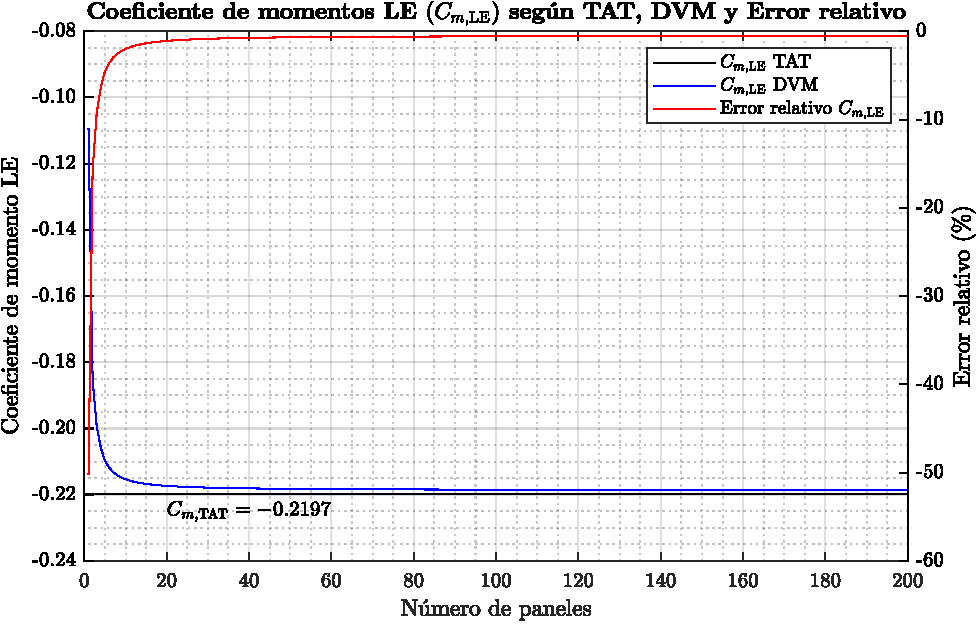
\includegraphics[width=\linewidth]{imagenes/verificacion2/verificacion_cmle.pdf}
    \caption{Coeficiente de momento respecto del LE $\left( C_{m,\text{LE}} \right)$ según TAT, DVM y error relativo en función del número de paneles $\left( N \right)$.}
    \label{fig:verificacion_cmle}
\end{figure}

El DVM proporciona una aproximación a la solución de la TAT. Por consiguiente, los resultados a obtener son los adquiridos con la teoría, \ie, $C_l = 0.6664$ y $C_{m,\text{LE}} = -0.2197$.

En la figura \ref{fig:verificacion_cl} se muestran el $C_l$ mediante TAT, la convergencia mediante DVM y el error relativo. Se aprecia que con pocos paneles se obtiene un error significativo, que disminuye a medida que $N$ aumenta. Para $N \geq 80$ el error es inferior al $0.5\%$, considerándose despreciable.

En la figura \ref{fig:verificacion_cmle} se muestran el $C_{m,\text{LE}}$ mediante TAT, la convergencia usando DVM y el error relativo. La relación entre el error y el número de paneles es idéntica a la del coeficiente de sustentación, \ie, el error disminuye rápidamente al aumentar el número de paneles.